\documentclass[11pt]{article}
\usepackage[left=1in, right=1in, top=1in, bottom=1in]{geometry}
\usepackage{amsmath, amssymb, amsfonts}
\usepackage{graphicx}
\usepackage{xcolor}
\usepackage{float}
\usepackage{tikz}
\usepackage{booktabs}

\begin{document}
	\begin{center}
	{\Large Mitigation model}	
	\end{center}
	
	\section{State variables and law of motion}
	
	Total capital:
	$$
	d \log K = (\mu_k + i - \frac{\kappa}{2} i^2 - \frac{\sigma_k^2}{2}) dt + \sigma_k dW
	$$
	
	Temperature anomaly:
	$$
	d Y = e(\theta_\ell dt + \varsigma dW)
	$$
	
	$R\& D$ investment, $X$, leads to an increased arrival rate of a one time jump in green sector productivity:
	$$
	d\log \mathcal{I}_g = - \zeta dt + \Psi_0 (\frac{X}{\mathcal{I}_g})^{\Psi_1} dt - \frac{\sigma_g^2}{2} dt + \sigma_g dW 
	$$
	
	Here we use $\Psi_1 = 1/2$
	
	Construct the following process:
	\begin{align*}
		\bar{Y}_t = \begin{cases}
			Y_t, & t \le \tau\\
			Y_t - Y_\tau + \bar{y}, & t > \tau
		\end{cases}
	\end{align*}
where $\tau$ is the date of the Poisson event.
	
	Log damages: 
	\begin{align*}
		\log N_t = \Gamma(\bar{Y}_t) + \iota_n \cdot Z_t
	\end{align*}

where
\begin{align*}
	\Gamma(y) = \gamma_1 y + \frac{\gamma_2}{2} y^2 + \frac{\gamma_3^{(m)}}{2} \mathbb{I}_{y \ge \bar{y}} (y - \bar{y})^2, \quad m = 1, 2, \dots, 20
\end{align*}

Damage jump intensity
\begin{align*}
	\mathcal{I}_d = \begin{cases}
		r_1 \left(\exp(\frac{r_2}{2} (Y - \underline{y})^2 ) - 1\right), & Y \ge \underline{y}\\
		0, & Y < \underline{y}
	\end{cases}
\end{align*}
	
	\section{Damage jump and technology jump}
	Suppose there are three technology states. Denote them as tech I, tech II and tech III. 
	And the curvature in the ``tail" of the damage function is only revealed when to decision-makers when a Poisson event is triggered. And technology change and damage curvature revelation are independent.
	
	The following graph serves as a illustration for notations of different solutions:
	\begin{figure}[H]
		\centering
	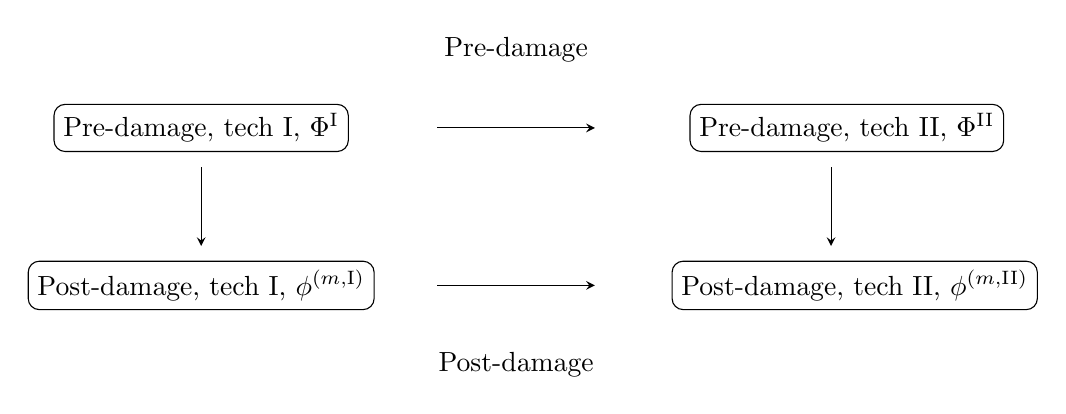
\begin{tikzpicture}
		\node[draw, rounded corners] at (2,2) {Pre-damage, tech I, $\Phi^{\text{I}}$};
		\draw[-stealth] (5,2) -- (7,2);
		\draw[-stealth] (2,1.5) -- (2,0.5);
%		\node[draw, rounded corners] at (6,2) {Pre-damage, tech II, $\Phi^{\text{II}}$};
%		\draw[-stealth] (8.5,2) -- (9.5,2);
%		\draw[-stealth] (6,1.5) -- (6,0.5);
		\node[draw, rounded corners] at (10.2,2) {Pre-damage, tech II, $\Phi^{\text{II}}$};
		\node at (6, 3) {Pre-damage};
		% POST DAMAGE
		\node[draw, rounded corners] at (2,0) {Post-damage, tech I, $\phi^{(m, \text{I})}$};
		\draw[-stealth] (5,0) -- (7,0);
%		\node[draw, rounded corners] at (6,0) {Post-damage, tech II, $\phi^{(m, \text{II})}$};
%		\draw[-stealth] (8.6,0) -- (9.5,0);
		\draw[-stealth] (10,1.5) -- (10,0.5);
		\node[draw, rounded corners] at (10.3,0) {Post-damage, tech II, $\phi^{(m, \text{II})}$};
		\node at (6, -1) {Post-damage};
%		\draw[color=gray] (-2, -1) rectangle ++(4,4);
	\end{tikzpicture}
		\caption{Damage jump and technology jump}
	\end{figure}

	\section{Post-damage, tech II}
	
	At tech III, $\bar\vartheta = 0$.
	For $m = 1,2,\dots, 20$, value function $V^{(m)} (\log K, Y, \log N)$
	\begin{align*} 
		0 = \max_{i,e} \min_{\omega_\ell:\sum_{\ell = 1}^L \omega_\ell = 1 } &   - \delta V^{(m)}(\log K,Y, \log N) +  \delta \log \left( \alpha - i -  \alpha \overline{\vartheta} \left[ 1 - \left(\frac {e} { \alpha \overline\lambda K} \right) \right]^\theta \right) - \delta \log N + \delta\log K \cr 
		& + \frac {\partial V^{(m)}}{\partial \log K} 
		\left[ \mu_k    + i   -
		{\frac { \kappa} 2} i^2  -  \frac  {|\sigma_k|^2}  2\right]  + \frac {|\sigma_k|^2} 2  \frac {\partial^2 V^{(m)}}{\partial \log K^2} \cr
		& + \frac {\partial  V^{(m)}}{\partial Y}  \sum_{\ell=1}^L \omega_\ell  \theta_\ell {e} + {\frac 1 2} \frac {\partial^2 V^{(m)}}{\partial Y^2} |\varsigma|^2 e^2  \cr
		& + \frac{\partial V^{(m)}}{\partial \log N} \left( \left[ \gamma_1 + \gamma_2 Y + \gamma_3^{(m)} \mathbb{I}_{Y > \bar{y}} (Y - \bar{y})\right]   \sum_{\ell=1}^L \omega_\ell \theta_\ell {e} + \frac{\gamma_2 + \gamma_3^{(m)}\mathbb{I}_{Y>\bar{y}}}{2} |\varsigma|^2  e^2 \right) \cr
		& + \frac{1}{2}\frac{\partial^2 V^{(m)}}{\partial \log N^2} \left[ \gamma_1 + \gamma_2 Y + \gamma_3^{(m)}\mathbb{I}_{Y > \bar{y}} (Y - \bar{y})\right]^2 |\varsigma|^2 e^2 \cr
		& + \xi_a \sum_{\ell = 1}^L \omega_\ell \left( \log \omega_\ell - \log \pi_\ell \right)
	\end{align*} 
	
	We simplify out $\log N$ by expressing the value function as  $V^{(m)} = \upsilon_d \log N + \phi^{(m)}(\log K, Y)$. 
	Therefore, $\upsilon_d=-1$ and $\frac{\partial^2 V^{(m)}}{\partial \log N^2} = 0$. And $\phi^{(m)}$ solves the following HJB:
\begin{align*} 
	0 = \max_{i,e}  &   - \delta \phi^{(m)}(\log K,Y) +  \delta \log \left( \alpha - i \right) + \delta\log K \cr 
	& + \frac {\partial \phi^{(m)}}{\partial \log K} 
	\left[ \mu_k    + i   - {\frac { \kappa} 2} i^2  -  \frac  {|\sigma_k|^2}  2\right]  + \frac {|\sigma_k|^2} 2  \frac {\partial^2 \phi^{(m)}}{\partial \log K^2}
\end{align*} 

Denote solutions in this section are $V^{(m, \text{III})}$ and $\phi^{(m, \text{III})}$.

\section{Post-damage, tech I}

	At tech I, $\bar\vartheta$ and $\bar\lambda$ pair use the following values:
	\begin{table}[H]
		\centering
		\begin{tabular}{lll}
			\toprule
			Tech state & $\bar\vartheta$ & $\bar \lambda$\\
			\midrule
			tech I & 0.04530 & 0.1206\\
			\bottomrule
		\end{tabular}
	\end{table}
And we add an additional state, $\log \mathcal{I}_g$ and an additional control variable $x = \frac{X}{K}$.
$X$ is the R\&D investment and $K$ is total capital.
	 
	 At tech II, for $m = 1,2,\dots, 20$, value function $V^{(m)} (\log K, Y, \log \mathcal{I}_g, \log N)$ and suppose Poisson event for damage function is triggered.
	\begin{align*} 
		0 = \max_{i,e,x} \min_{\omega_\ell:\sum_{\ell = 1}^L \omega_\ell = 1 }\min_{g >0} &   - \delta V^{(m)}(\log K,Y,\log \mathcal{I}_g, \log N) +  \delta \log \left( \alpha - i -  \alpha \overline{\vartheta} \left[ 1 - \left(\frac {e} { \alpha \overline\lambda K} \right) \right]^\theta -x\right)\\
		& - \delta \log N + \delta\log K \cr 
		& + \frac {\partial V^{(m)}}{\partial \log K} 
		\left[ \mu_k    + i   -
		{\frac { \kappa} 2} i^2  -  \frac  {|\sigma_k|^2}  2\right]  + \frac {|\sigma_k|^2} 2  \frac {\partial^2 V^{(m)}}{\partial \log K^2} \cr
		& + \frac {\partial  V^{(m)}}{\partial Y}  \sum_{\ell=1}^L \omega_\ell  \theta_\ell {e} + {\frac 1 2} \frac {\partial^2 V^{(m)}}{\partial Y^2} |\varsigma|^2 e^2  \cr
		& +\textcolor{blue}{ \frac{\partial V^{(m)}}{\partial \log \mathcal{I}_g} (- \zeta + \Psi_0 (x\frac{K}{\mathcal{I}_g})^{\Psi_1} - \frac{\sigma_g^2}{2} ) + \frac{\sigma_g^2}{2}\frac{\partial^2 V^{(m)}}{\partial \log \mathcal{I}_g^2}} \tag*{[additional state]}\\
		& + \frac{\partial V^{(m)}}{\partial \log N} \left( \left[ \gamma_1 + \gamma_2 Y + \gamma_3^{(m)} \mathbb{I}_{Y > \bar{y}} (Y - \bar{y})\right]   \sum_{\ell=1}^L \omega_\ell \theta_\ell {e} + \frac{\gamma_2 + \gamma_3^{(m)}\mathbb{I}_{Y>\bar{y}}}{2} |\varsigma|^2  e^2 \right) \cr
		& + \frac{1}{2}\frac{\partial^2 V^{(m)}}{\partial \log N^2} \left[ \gamma_1 + \gamma_2 Y + \gamma_3^{(m)} \mathbb{I}_{Y > \bar{y}} (Y - \bar{y})\right]^2 |\varsigma|^2 e^2 \cr
		& + \xi_a \sum_{\ell = 1}^L \omega_\ell \left( \log \omega_\ell - \log \pi_\ell \right)\\
		& +\textcolor{blue}{ \xi_g \mathcal{I}_g \left(1 - g + g  \log(g) \right) + \mathcal{I}_g g (V^{(m, \text{III})} - V^{(m)} )} \tag*{[robustness concern]}
	\end{align*} 
	
	We simplify out $\log N$ by similarly expressing the value function as  $V^{(m)} = \upsilon_d \log N + \phi^{(m)}(\log K, Y, \log \mathcal{I}_g)$. 
	Therefore, $\upsilon_d=-1$ and $\frac{\partial^2 V^{(m)}}{\partial \log N^2} = 0$. And $\phi^{(m)}(\log K,Y, \log \mathcal{I}_g)$ solves the following HJB:
	\begin{align*} 
		0 = \max_{i,e, x} \min_{\omega_\ell:\sum_{\ell = 1}^L \omega_\ell = 1 } \min_{g>0} &   - \delta \phi^{(m)}(\log K,Y, \log \mathcal{I}_g) +  \delta \log \left( \alpha - i -  \alpha \overline{\vartheta} \left[ 1 - \left(\frac {e} { \alpha \overline\lambda K} \right) \right]^\theta - x\right) + \delta\log K \cr 
		& + \frac {\partial \phi^{(m)}}{\partial \log K} 
		\left[ \mu_k    + i   - {\frac { \kappa} 2} i^2  -  \frac  {|\sigma_k|^2}  2\right]  + \frac {|\sigma_k|^2} 2  \frac {\partial^2 \phi^{(m)}}{\partial \log K^2} \cr
		& + \frac {\partial \phi^{(m)}}{\partial Y}  \sum_{\ell=1}^L \omega_\ell  \theta_\ell {e} + {\frac 1 2} \frac {\partial^2 \phi^{(m)}}{\partial Y^2} |\varsigma|^2 e^2  \cr
		& +\textcolor{blue}{ \frac{\partial \phi^{(m)}}{\partial \log \mathcal{I}_g} (- \zeta + \Psi_0 (x\frac{K}{\mathcal{I}_g})^{\Psi_1} - \frac{\sigma_g^2}{2} ) + \frac{\sigma_g^2}{2}\frac{\partial^2 \phi^{(m)}}{\partial \log \mathcal{I}_g^2}} \\
		& - \left( \left[ \gamma_1 + \gamma_2 Y + \gamma_3^{(m)} \mathbb{I}_{Y > \bar{y}} (Y - \bar{y})\right]   \sum_{\ell=1}^L \omega_\ell \theta_\ell {e} + \frac{\gamma_2 + \gamma_3^{(m)}\mathbb{I}_{Y>\bar{y}}}{2} |\varsigma|^2  e^2 \right) \cr
		& + \xi_a \sum_{\ell = 1}^L \omega_\ell \left( \log \omega_\ell - \log \pi_\ell \right)\\
	& +\textcolor{blue}{ \xi_g \mathcal{I}_g \left(1 - g + g  \log(g) \right) + \mathcal{I}_g g (\phi^{(m, \text{III})} - \phi^{(m)} )}
	\end{align*} 
Denote post-damage tech II value functions solved from above HJBs as  $V^{(m, \text{II})}$ and $\phi^{(m, \text{II})}$. We can solve for $V^{(m, \text{I})}$ and $\phi^{(m, \text{I})}$ by changing the values of $\bar\vartheta$ and $\bar\lambda$.

	\section{Pre-damage and pre technology jump (tech I) HJB}
	Denote $x = \frac{X}{K}$ as R\& D invesment - total capital ratio, and there are two technology jumps. 
	
	Given pre-damage tech II value function $\mathcal{V}^{\text{II}}(\log K,Y, \log \mathcal{I}_g, \log N)$,  value function $\mathcal{V}(\log K,Y, \log \mathcal{I}_g, \log N)$ with 4 state variables solve for the following pre damage jump and pre technology jump HJB:
		\begin{align*} 
		0 = \max_{i,e,x} \min_{\omega_\ell, \sum_{\ell = 1}^L \omega_\ell = 1, g, g_m } &   - \delta \mathcal{V}(\log K,Y, \log \mathcal{I}_g, \log N) +  \delta \log \left( \alpha - i -  \alpha \overline{\vartheta} \left[ 1 - \left(\frac {e} { \alpha \overline\lambda K} \right) \right]^\theta  - x \right)\\
		& - \delta \log N + \delta\log K \cr 
		& + \frac {\partial \mathcal{V}}{\partial \log K} 
		\left[ \mu_k    + i   -
		{\frac { \kappa} 2} i^2  -  \frac  {|\sigma_k|^2}  2\right]  + \frac {|\sigma_k|^2} 2  \frac {\partial^2 \mathcal{V}}{\partial \log K^2} \cr
		& + \frac {\partial  \mathcal{V}}{\partial Y}  \sum_{\ell=1}^L \omega_\ell  \theta_\ell {e} + {\frac 1 2} \frac {\partial^2 \mathcal{V}}{\partial Y^2} |\varsigma|^2 e^2  \cr
		& + \frac{\partial \mathcal{V}}{\partial \log \mathcal{I}_g} (- \zeta + \Psi_0 (x\frac{K}{\mathcal{I}_g})^{\Psi_1} - \frac{\sigma_g^2}{2} ) + \frac{\sigma_g^2}{2}\frac{\partial^2 \mathcal{V}}{\partial \log \mathcal{I}_g^2} \\
		& + \frac{\partial \mathcal{V}}{\partial \log N} \left( \left[ \gamma_1 + \gamma_2 Y\right]   \sum_{\ell=1}^L \omega_\ell \theta_\ell {e} + \frac{\gamma_2}{2} |\varsigma|^2  e^2 \right) \cr
		& + \frac{1}{2}\frac{\partial^2 \mathcal{V}}{\partial \log N^2} \left[ \gamma_1 + \gamma_2 Y\right]^2 |\varsigma|^2 e^2 \cr
		& + \xi_a \sum_{\ell = 1}^L \omega_\ell \left( \log \omega_\ell - \log \pi_\ell \right) \\
		& + \xi_g \mathcal{I}_g \left(1 - g + g  \log(g) \right) + \mathcal{I}_g g (\mathcal{V}^{\text{II}} - \mathcal{V} )\\
		&  + \xi_d \mathcal{I}_d \sum_{m=1}^M \pi_d^m(1 - g_m + g_m \log(g_m))+ \mathcal{I}_d\sum_{m=1}^M \pi_d^m g_m (V^{(m, \text{II})} - \mathcal{V})
	\end{align*} 

	We simplify out $\log N$ by similarly expressing the pre-damage value function as  $\mathcal{V} = \upsilon_d \log N + \Phi(\log K, Y, \log \mathcal{I}_g)$. 
Therefore, $\upsilon_d=-1$ and $\frac{\partial^2 \mathcal{V}}{\partial \log N^2} = 0$. And $\Phi(\log K,Y, \log \mathcal{I}_g)$ solves the following HJB:
	
	\begin{align*} 
		0 = \max_{i,e,x} \min_{\omega_\ell, \sum_{\ell = 1}^L \omega_\ell = 1, g, g_m } &   - \delta \Phi(\log K,Y, \log \mathcal{I}_g) +  \delta \log \left( \alpha - i -  \alpha \overline{\vartheta} \left[ 1 - \left(\frac {e} { \alpha \overline\lambda K} \right) \right]^\theta  - x \right) + \delta\log K \cr 
		& + \frac {\partial \Phi}{\partial \log K} 
		\left[ \mu_k    + i   -
		{\frac { \kappa} 2} i^2  -  \frac  {|\sigma_k|^2}  2\right]  + \frac {|\sigma_k|^2} 2  \frac {\partial^2 \Phi}{\partial \log K^2} \cr
		& + \frac {\partial \Phi}{\partial Y}  \sum_{\ell=1}^L \omega_\ell  \theta_\ell {e} + {\frac 1 2} \frac {\partial^2\Phi}{\partial Y^2} |\varsigma|^2 e^2  \cr
		& + \frac{\partial V}{\partial \log \mathcal{I}_g} (- \zeta + \Psi_0 (x\frac{K}{\mathcal{I}_g})^{\Psi_1} - \frac{\sigma_g^2}{2} ) + \frac{\sigma_g^2}{2}\frac{\partial^2 V}{\partial \log \mathcal{I}_g^2} \\
		& - \left( \left[ \gamma_1 + \gamma_2 Y\right]   \sum_{\ell=1}^L \omega_\ell \theta_\ell { e} + \frac {\gamma_2} {2}|\varsigma|^2  e^2 \right) \cr
		& + \xi_a \sum_{\ell = 1}^L \omega_\ell \left( \log \omega_\ell - \log \pi_\ell \right) \\
		& + \xi_g \mathcal{I}_g \left(1 - g + g  \log(g) \right) + \mathcal{I}_g g (\Phi^{\text{II}} - \Phi)\\
		&  + \xi_d \mathcal{I}_d \sum_{m=1}^M \pi_d g_m (1 - g_m + g_m \log(g_m)) + \mathcal{I}_d \sum_{m=1}^M \pi_d^m g_m (\phi^{(m, \text{II})} - \Phi)
	\end{align*} 
	Denote pre-damage tech I value functions solved from above HJBs as  $\mathcal{V}^{\text{I}}$ and $\Phi^{\text{I}}$.
	
	
	\section{Uncertainty parameter configuration}
	\begin{itemize}
		\item Smooth ambiguity: $\xi_a$
		\item Damage uncertainty, $\xi_d$,
		\item Technology jump uncertainty, $\xi_g$
	\end{itemize}
	
	\begin{table}[H]
		\centering
		\begin{tabular}{llll}
			\toprule
			& $\xi_a$ & $\xi_d$ & $\xi_g$ \\
			\midrule
			baseline & $\infty$ & $\infty$ & $\infty$\\
			case 1 & $2 \times 10^{-4}$ & 0.050 & 0.050 \\
			case 2 & $2 \times 10^{-4}$ & 0.025& 0.025\\
			\bottomrule
		\end{tabular}
	\end{table}

\section{Pathway comparisons, with 20 damage functions}

\subsection{pre damage jump, pre technology jump R\& D investment}
\begin{figure}[H]
	\centering
	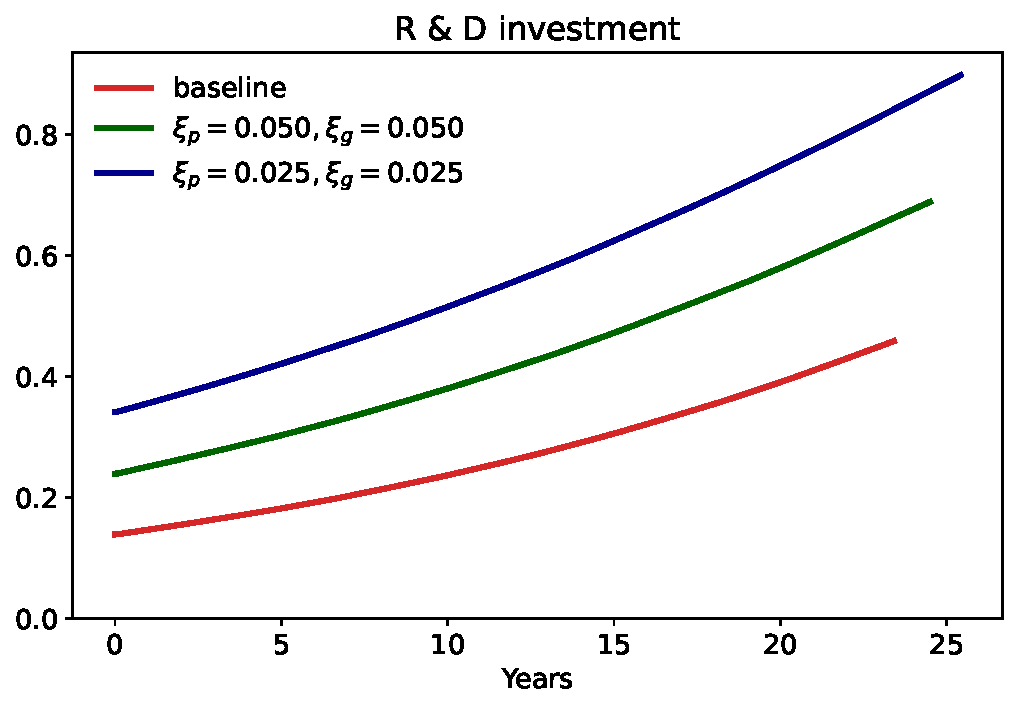
\includegraphics[width=\textwidth]{../figures/20damage/Xt_1p5.pdf}
	\caption{R \& D investment, pathways stop when temperature anomaly hits $1.5^o C$}
\end{figure}

\subsection{pre damage jump, pre technology jump emission}
\begin{figure}[H]
	\centering
	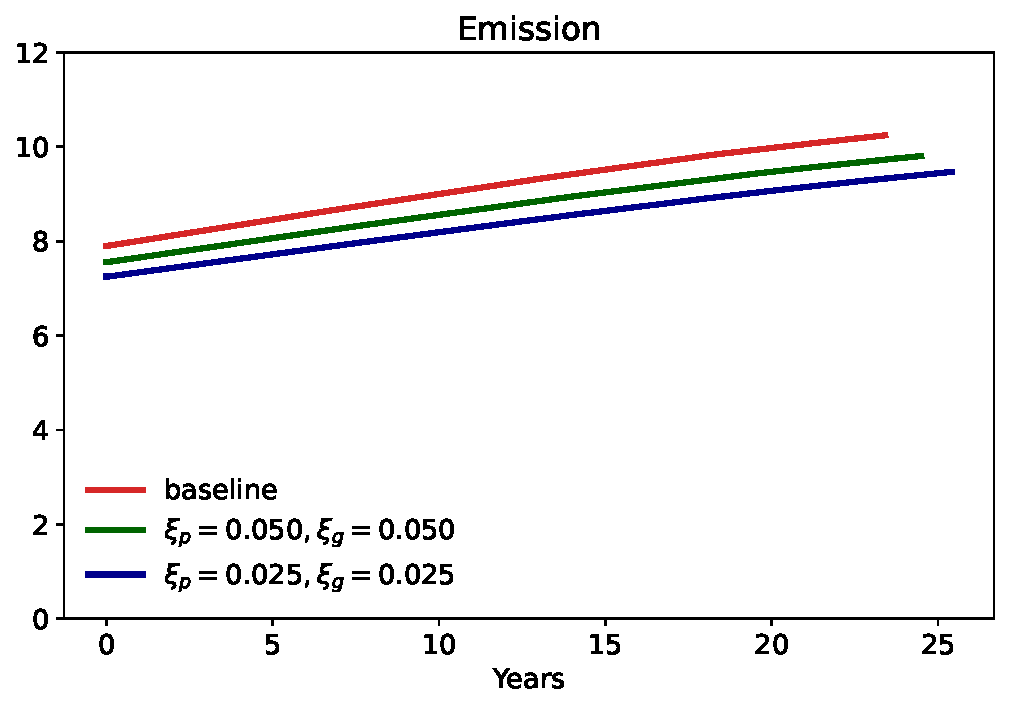
\includegraphics[width=\textwidth]{../figures/20damage/Et_1p5.pdf}
	\caption{Emission, pathways stop when temperature anomaly hits $1.5^o C$}
\end{figure}

\subsection{pre damage jump, pre technology jump temperature anomaly}
\begin{figure}[H]
	\centering
	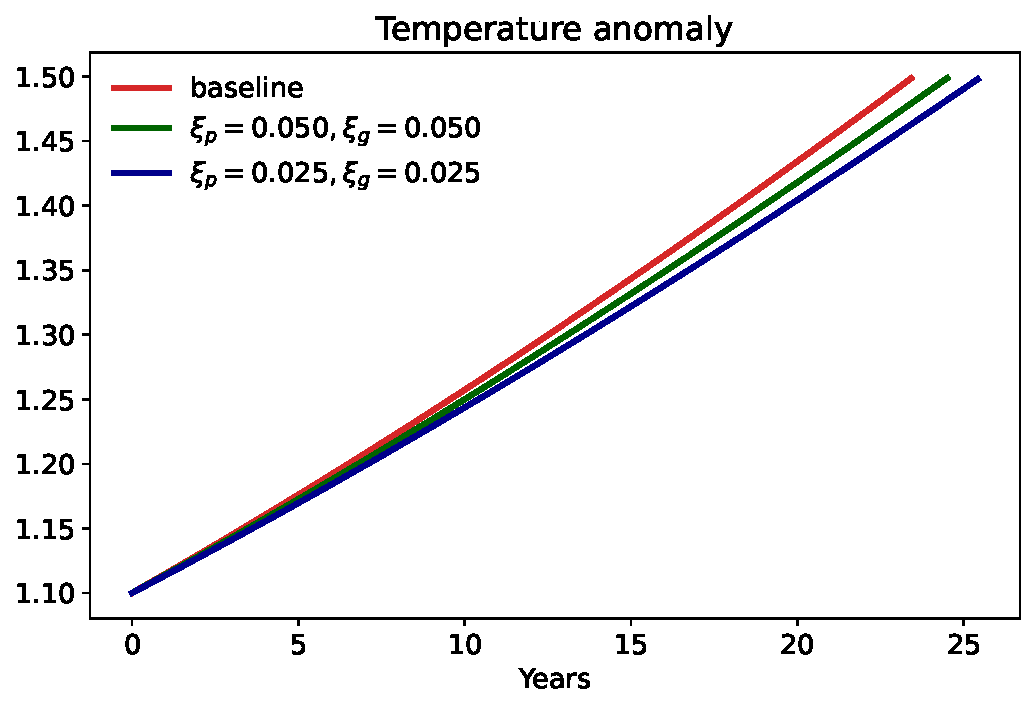
\includegraphics[width=\textwidth]{../figures/20damage/Yt_1p5.pdf}
	\caption{Temperature anomaly, pathways stop when temperature anomaly hits $1.5^o C$}
\end{figure}

\subsection{pre damage jump, pre technology jump technology jump intensity, $\mathcal{I}_g$}
\begin{figure}[H]
	\centering
	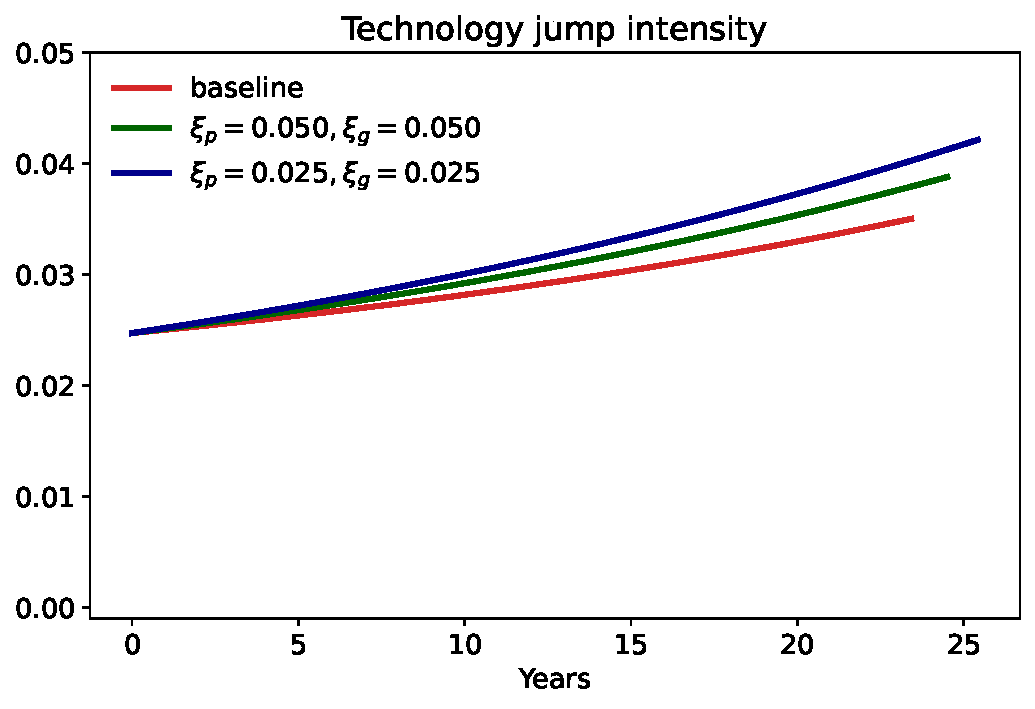
\includegraphics[width=\textwidth]{../figures/20damage/Lt_1p5.pdf}
	\caption{Technology jump intensity, $\mathcal{I}_g$, pathways stop when temperature anomaly hits $1.5^o C$}
\end{figure}

\section{Jump probabilities and distorted probabilities}

\subsection{Distorted probability of Poisson events for technology changes with different uncertainty configurations}


\begin{figure}[H]
	\centering
	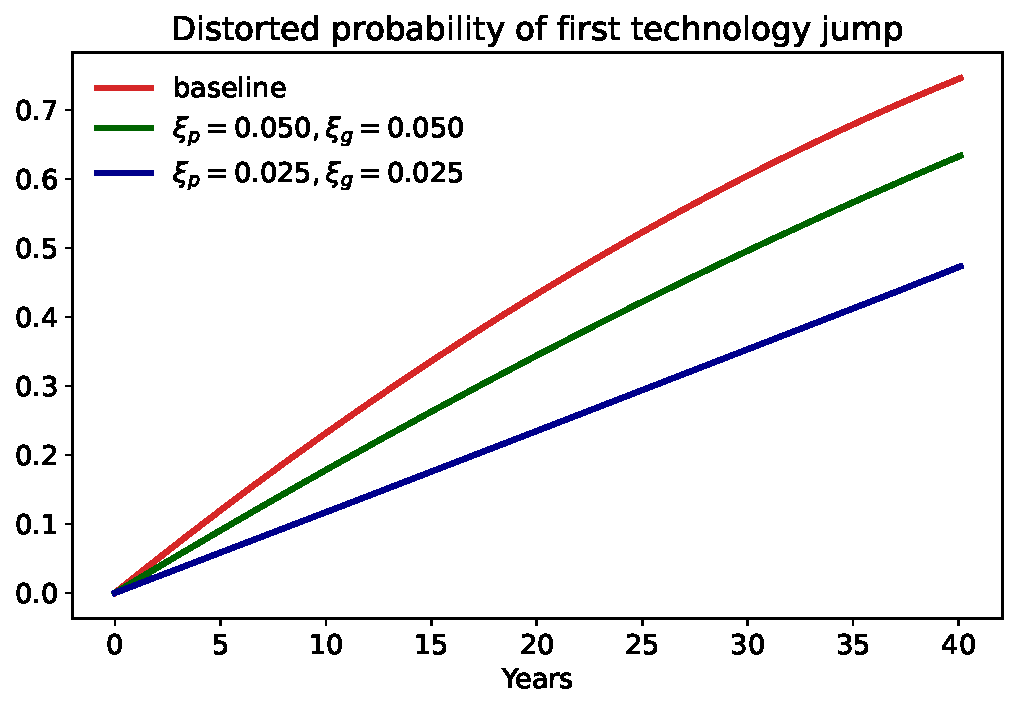
\includegraphics[width=0.85\textwidth]{../figures/20damage/Tech_jump_first.pdf}
\end{figure}

\begin{figure}[H]
	\centering
	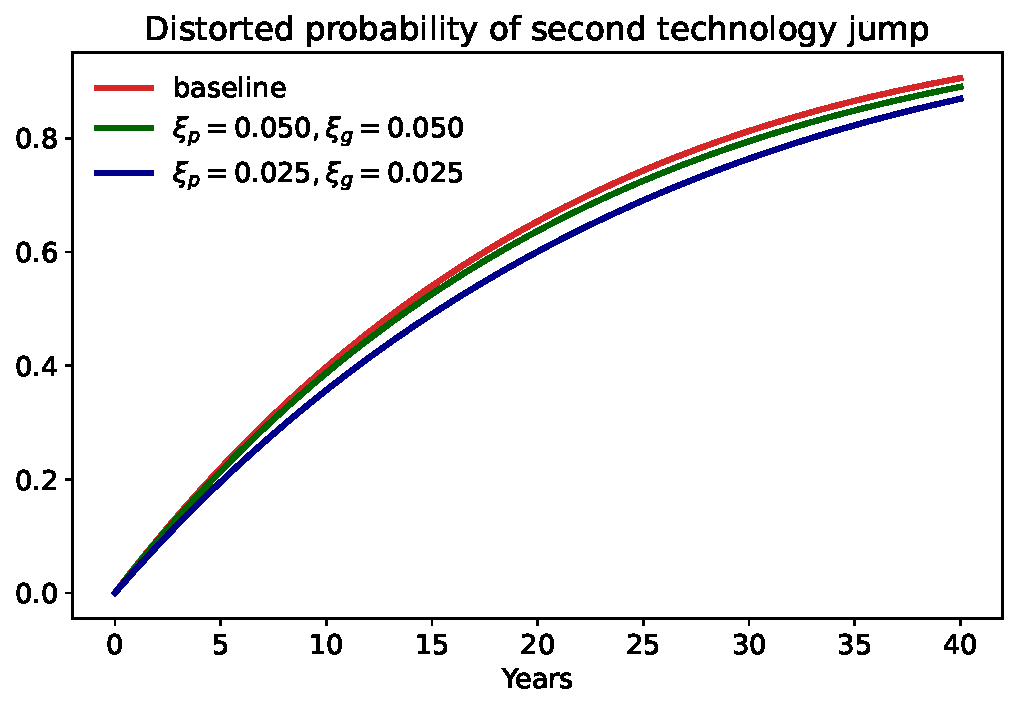
\includegraphics[width=0.85\textwidth]{../figures/20damage/Tech_jump_second.pdf}
\end{figure}

\subsection{Distorted probability of Poisson events for damage with different uncertainty configurations}


\begin{figure}[H]
	\centering
	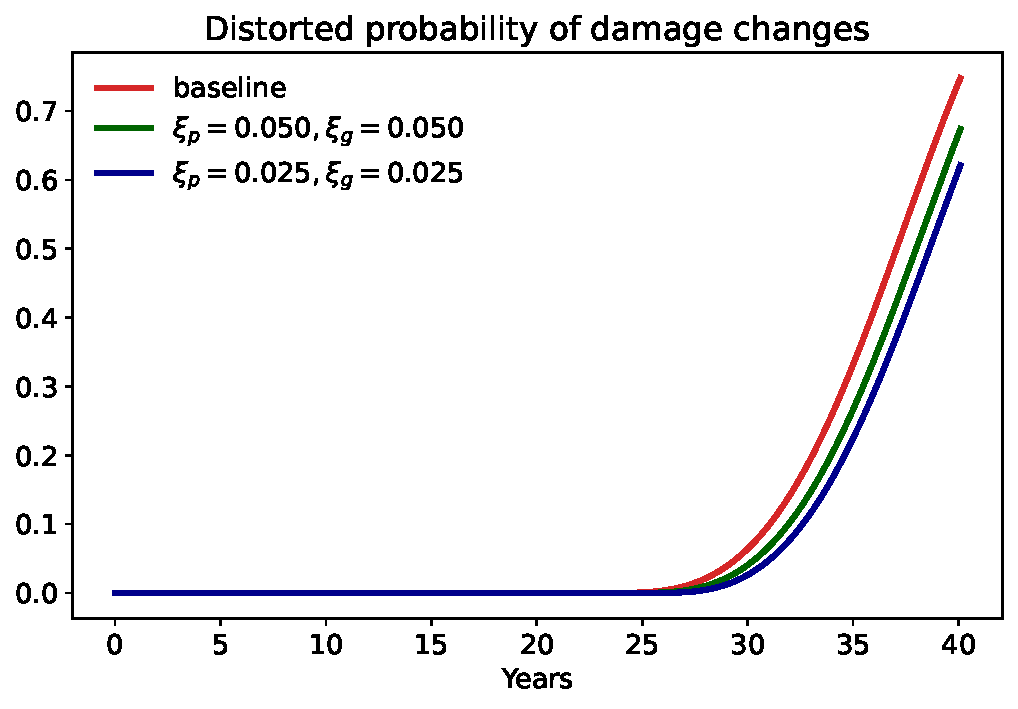
\includegraphics[width=0.85\textwidth]{../figures/20damage/Damage_prob.pdf}
\end{figure}

\subsection{Probability distortion for damage function, with $\xi_a = 2\times 10^{-4}$, $\xi_d = 0.05$ and $\xi_g = 0.05$}

\begin{figure}[H]
	\centering
	\includegraphics[width=0.85\textwidth]{../figures/20damage/Damage_distort.pdf}
	\caption{Red bars are for baseline probability, and blue bars are for distorted probability}
\end{figure}

\subsection{Probability distortion for climate sensitivity models, with $\xi_a = 2\times 10^{-4}$, $\xi_d = 0.05$ and $\xi_g = 0.05$}

\begin{figure}[H]
	\centering
	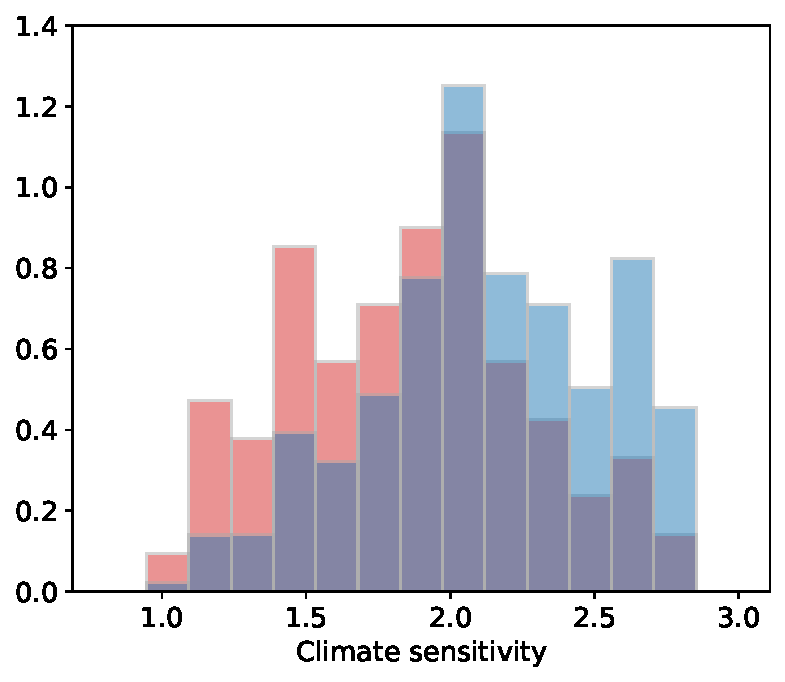
\includegraphics[width=0.85\textwidth]{../figures/20damage/worstcase.pdf}
		\caption{Red bars are for baseline density, and blue bars are for distorted density of climate sensitivity models}
\end{figure}
\end{document}